\chapter{Methods}

%\section{Methods}
\section{Aggregating Network Data}\label{sec:aggregdata}
TCR network repertoire varies in structure and sizes across different subjects and are continually shaping even for the same subject. This heterogeneous nature of the TCR repertoire data renders the dataset unfit for direct statistical inferences. The technique used to handle this heterogeneity is accomplished by aggregating the TCR network repertoire data for each patient. Summary statistics of these network properties were deduced per subject which were then considered as explanatory variables. The derived summary statistics largely consisted of Minimum, $1^{st}$ Quartile $(Q_1)$, Median, Mean, $3^{rd}$ Quartile $(Q_3)$ and Maximum data points. These summary statistics helped with generating a holistic view of the TCR network properties for the patients belonging to the two cohorts (longer and shorter overall survival).\par
Certain network properties also contained a significant number of \lq NA' values. For those properties along with computing the set of summary statistics (Min, $Q_1$, Median, Mean, $Q_3$ and Max) for the not null (or \lq NA') rows, the probability of those value being \lq NA' was also computed. Feature blocks were then created by collectively considering the summary statistics (including \lq prob(NA)') from the network data for each patient. This technique allowed us to represent the heterogeneous network data between the two groups of patients efficiently. Using this aggregated form of network data, we could then perform comparison of the network properties, run feature selection techniques, and also use this data to aid with simulation of the network property data discussed in the later sections.\par
\begin{table}[h]
\centering
\caption{Aggregated Transitivity data for a Patient }
\begin{tabular}{|c|c|c|c|c|c|c|}
\hline
\cellcolor[HTML]{D9E1F2}prob(NA) & \cellcolor[HTML]{D9E1F2}Min & \cellcolor[HTML]{D9E1F2}Q1 & \cellcolor[HTML]{D9E1F2}Median & \cellcolor[HTML]{D9E1F2}Mean  & \cellcolor[HTML]{D9E1F2}Q3    & \cellcolor[HTML]{D9E1F2}Max \\
\hline
0.698  & 0   & 0  & 0      & 0.141 & 0.201 & 1\\ \hline
\end{tabular}
\label{tab:aggreg_transitivity}
\end{table}

\autoref{tab:aggreg_transitivity} is a representation of the summary statistics of \lq Transitivity', a network property, which was aggregated for a single patient. \lq Transitivity' has a significant number of values as \lq NA' values, therefore, prob(NA) was computed. The entire list of summary statistics for all the network properties is provided in \autoref{tab:ntwrk_features}. The derived features were indexed individually (as \lq Feature Index' column) as well as collectively (column \lq Group') to feed these aggregated features to various variable selection models.
\begin{table}[H]
\caption{TCR Network Properties, corresponding Feature Blocks, Feature Indexes and Group indexes.}
\resizebox{\textwidth}{!}{%
\begin{tabular}{|
>{\columncolor[HTML]{EAEAEA}}c |c|c|c|}
\hline
\cellcolor[HTML]{D9E1F2}\textbf{Properties} &
  \cellcolor[HTML]{D9E1F2}\textbf{Feature Blocks} &
  \cellcolor[HTML]{D9E1F2}\textbf{Feature Index} &
  \multicolumn{1}{c|}{\cellcolor[HTML]{D9E1F2}\textbf{Groups}} \\ \hline
membership           & \# of clusters                                  & 1     & 1  \\ \hline
node\_count          & Min, Q1, Median (Q2),   Mean, Q3, Max           & 2-7   & 2  \\ \hline
deg                  & Min, Q1, Median (Q2),   Mean, Q3, Max           & 8-13  & 3  \\ \hline
AA\_length           & Min, Q1, Median (Q2),   Mean, Q3, Max           & 14-19 & 4  \\ \hline
Count\_PRE\_INFUSION & Min, Q1, Median (Q2),   Mean, Q3, Max           & 20-25 & 5  \\ \hline
Count\_DOSE\_2       & Min, Q1, Median (Q2),   Mean, Q3, Max           & 26-31 & 6  \\ \hline
deg\_avg             & Min, Q1, Median (Q2),   Mean, Q3, Max           & 32-37 & 7  \\ \hline
diam\_length         & Min, Q1, Median (Q2),   Mean, Q3, Max           & 38-43 & 8  \\ \hline
assortativity        & prob(NA), Min, Q1,   Median (Q2), Mean, Q3, Max & 44-50 & 9  \\ \hline
transitivity         & prob(NA), Min, Q1,   Median (Q2), Mean, Q3, Max & 51-57 & 10 \\ \hline
edge\_density        & Min, Q1, Median (Q2),   Mean, Q3, Max           & 58-63 & 11 \\ \hline
centr\_degree        & Min, Q1, Median (Q2),   Mean, Q3, Max           & 64-69 & 12 \\ \hline
centr\_clo           & prob(NA), Min, Q1,   Median (Q2), Mean, Q3, Max & 70-76 & 13 \\ \hline
eigen\_centrality    & Min, Q1, Median (Q2),   Mean, Q3, Max           & 77-82 & 14 \\ \hline
centr\_eigen         & prob(NA), Min, Q1,   Median (Q2), Mean, Q3, Max & 83-89 & 15 \\ \hline
\end{tabular}}
\label{tab:ntwrk_features}
\end{table}

Using the aggregation strategy, the entire TCR network data was consolidated in a manner such that a single layer of information exists for each patient. \autoref{tab:sample_aggreg_data} is a snapshot of the aggregated network data layout for a single patient. The resultant data set consists of 89 network features (individual summary statistics) and 15 network properties (aggregated summary statistics). Based on the variable selection models, either the network features or the network properties would be used. 

\begin{table}[H]
\caption{Aggregated Network Data Layout for a Patient}
\resizebox{\textwidth}{!}{%
\begin{tabular}{|c|c|c|c|c|}
\hline
\rowcolor[HTML]{D9E1F2} 
\textbf{}                         & \textbf{Membership} & \textbf{Node\_Count}             & \textbf{…}   & \textbf{Centr\_Eigen}                      \\ \hline
\cellcolor[HTML]{EAEAEA}Patient-1 & \# of clusters      & Min, Q1, Median, Mean, Q3, Max & (..),..,(..) & prob(NA), Min, Q1, Median, Mean, Q3, Max \\ \hline
\end{tabular}}
\label{tab:sample_aggreg_data}
\end{table}

\section{Models}\label{sec:models}
Prioritizing the TCR network properties and selecting the most significant network signatures using the TCR repertoire data is the primary contribution of this work. In the previous section we were able to aggregate the network property data in a systematic manner so that statistical inferences can now be drawn on them. In literature there are three most popular Variable Selection techniques --- Filter method, Wrapper method and Embedded method. The Filter method picks up the intrinsic properties of the explanatory variables (i.e., their correlation with the response variable) measured via univariate statistics instead of cross-validation performance. This method ignores feature dependencies and has no interactions with the classification model for variable selection. The Wrapper method attempts to find the optimal variable subset by iteratively selecting the variables based on the classifier performance. This technique, even though it considers variable dependencies, becomes computationally heavy (even impossible) in case of high dimensional feature space and is easily susceptible to overfitting. For our work we consider the Embedded method which combines the qualities of the Filter and the Wrapper methods while overcoming their respective limitations. Embedded method is the most preferred variable selection technique when handling high-dimensional genetic data.\par
We implement the following embedded techniques and compare their performances --- Lasso (\cite{tibshir}Tibshirani, 1996), Group Lasso (\cite{grouporigin}Yuan and Lin, 2005), and Exclusive Lasso (\cite{exclusv_lasso}Zhou, Jin and Hoi, 2010). The \autoref{fig:model_general} gives us a general idea of how these three variable Selection methods work.\par

 In Lasso the objective function penalizes the absolute size of the regression coefficients, based on the value of a tuning parameter $\lambda$. In doing so, Lasso can drive the coefficients of irrelevant variables to zero, thus performing automatic variable selection. We will deploy Lasso for selecting top network features in subsequent sections. Prior to that we implement the Group Lasso model, an extension of the Lasso, that performs variable selection on grouped variables (feature blocks). Group Lasso is known to perform better when predictors are not
distinct but arise from common underlying factors. In our case, a set of aggregated features (a feature block) is derived from the same parent network feature which may have some \lq relevance' among themselves. Using Group Lasso we try to prioritize the prominent network properties as a whole. Finally, we will use Exclusive Lasso to dissect each feature block and find their most significant summary statistics.
\autoref{fig:model_general} shows how Lasso, Group Lasso and Exclusive Lasso perform variable selection. The Lasso is indifferent to the aggregated group structure (feature blocks) created for the network properties. In the Group Lasso, feature blocks compete among themselves ($L_1$ norm between feature blocks) and the most significant feature blocks (all sub features inclusive) are selected. The Exclusive Lasso enforces the $L_2$ norm among different feature blocks and the $L_1$ norm between the features in a single block. As a result, at least one feature is selected from each of the feature blocks.\par

\begin{figure}[H]
\centering
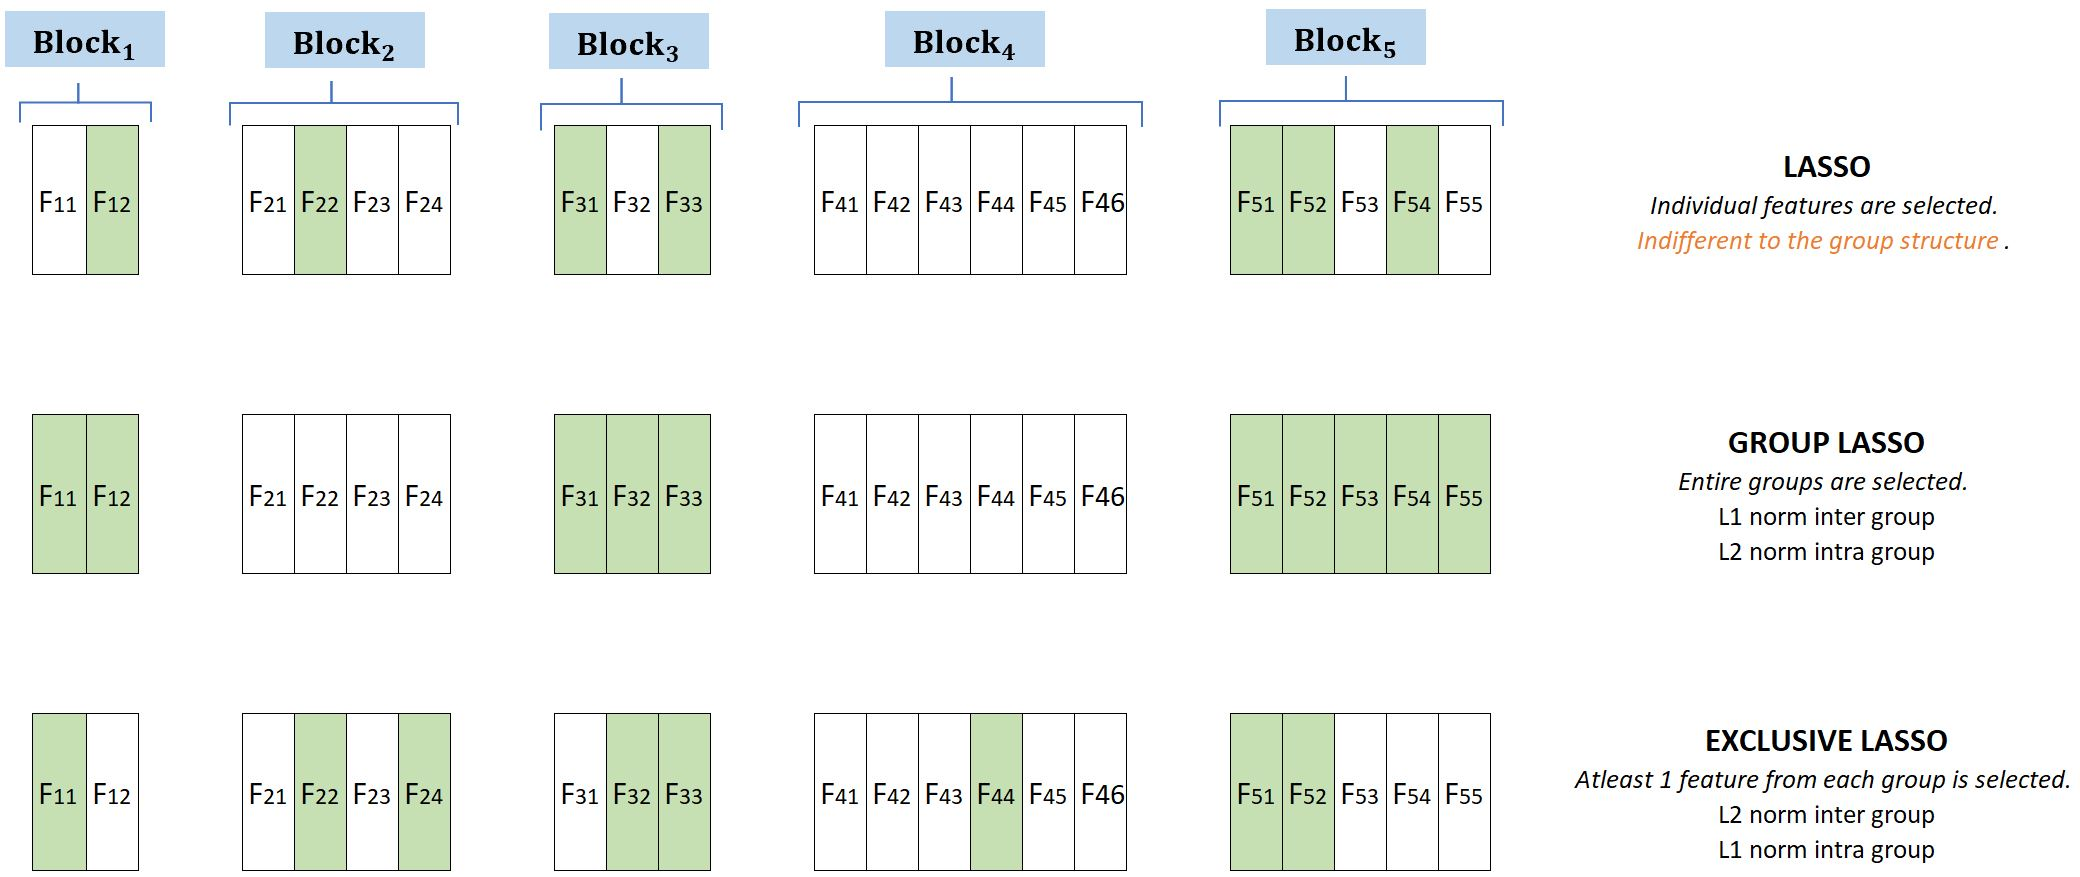
\includegraphics[scale=0.65]{Model_general.jpg}
\caption{General Behaviour for Lasso, Group Lasso and Exclusive Lasso.}%
{$\text{Block}_{(i)}$ represents the $i^{th}$ feature block (TCR network property) and $F_{ij}$ represents the summary statistics derived for the $i^{th}$ feature block.}
\label{fig:model_general}
\end{figure}
\section{Prioritizing Network Properties}\label{sec:priorntw}
We use the Group Lasso variable selection technique to identify the significant TCR network properties (feature blocks) that help to differentiate between patients belonging to the longer and the shorter overall survival cohorts.
\subsection{Logistic Group Lasso Model set-up}\label{subsec:grouplasso}
Assume that we have independent and identically distributed observations $(\mathbf{x}_i, y_i)$ where $i=1, . . . , n$ of a $p$-dimensional vector $\mathbf{x}_i \in \mathbb{R}^p$ and a binary 
$y=(y_1,...,y_n)^T$ as the binary outcomes ($y_i \in{0,1}$) for all the n observations. For this work, $n=65$ (\# of patients) and $p=15$ (\# of explanatory variables). The response variable $y_i=1$ denotes $OS\_mon\ge 20.3$ - patient belongs to the \lq longer overall survival' group, and $y_i=0$ denotes $OS\_mon< 20.3$ - patient belongs to the \lq shorter overall survival' group. The predictors can be written as $\mathbf{x}_i = ({x}_{i1}, ...,{x}_{ip})^T$ which are then grouped (based on some known common factors between the features) to form a total of $G$ groups of predictors. In this study, the summary statistics derived from a single network property are grouped together to form a feature block. The degrees of freedom is denoted as $\text{df}_g$ of the $g^{\text{th}}$ predictor group. The predictor variables can be rewritten as $\mathbf{x}_i=(\mathbf{x}_{i1}, ..., \mathbf{x}_{iG})^T$ using the grouped variables $\mathbf{x}_{ig}\in\mathbb{R}^{\text{df}_g}$ where $g=1, ..., G$.\par
Applying the latter representation of the predictor variables, the log of odds (logit) for the logistic regression model can be written as:
\begin{equation}\label{eq:1}
\log\{\frac{p_{\pmb{\beta}}(\mathbf{x}_i)}{1-p_{\pmb{\beta}}(\mathbf{x}_i)}\}=\eta_{\pmb{\beta}}(\mathbf{x}_i)
\end{equation}
where $p_{\pmb{\beta}}(\mathbf{x}_i) = \mathbb{P}_{\pmb{\beta}}(y_i=1|\mathbf{x}_i)$ and $\eta_{\pmb{\beta}}(\mathbf{x}_i) = \beta_0+\sum_{g=1}^{G}\mathbf{x}_{ig}^T\beta_g$. Here $\pmb{\beta}=(\beta_0,\beta_1, .., \beta_G)^T$ are the coefficients for the $G$ grouped predictors.\par
The logistic group lasso estimator $\pmb{\hat\beta_{\lambda}}$ is derived by minimizing the objective function:
\begin{equation}\label{eq:2}
S_{\lambda}(\pmb{\beta}) = -l(\pmb{\beta})+\lambda\sum_{g=1}^{G} s(\text{df}_g)\|\beta_g\|_2^1
\end{equation}
where $l(.)$ is the log-likelihood function and is given as
\begin{equation*}
L(\pmb{\beta})= \Pi_{i=1}^{n}(p_{\pmb{\beta}}(\mathbf{x}_i))^{y_i}(1-p_{\pmb{\beta}}(\mathbf{x}_i))^{1-y_i}
\end{equation*}
\begin{equation}\label{eq:3}
l(\pmb{\beta})=\log[L(\pmb{\beta})]=\sum_{i=1}^{n}[y_i\eta_{\pmb{\beta}}(\mathbf{x}_i)-\log(1+\exp(\eta_{\pmb{\beta}}(\mathbf{x}_i))]
\end{equation}
and the penalty function is given as
\begin{equation}\label{eq:grp_penal}
\lambda\sum_{g=1}^{G} s(\text{df}_g)\|\beta_g\|_2^1
\end{equation}
In the equation \eqref{eq:2}, the tuning parameter $\lambda\ge 0$ controls the amount of penalization and is subject to $\sum_{g=1}^{G}\|\beta_g\|_2^1\le \theta(\lambda)$ where $\theta(.)$ is some function of $\lambda$. In the penalty function equation \eqref{eq:grp_penal}, $\|\beta_g\|_2^1$ implies the $L_1-$norm inter-group and the $L_2-$norm intra-group. The function $s(.)$ is used to rescale the penalty with respect to the dimensionality of the parameter vector $\beta_g$ (\cite{grouporigin}Yuan and Lin, 2006).\par
An optimal value for the tuning parameter $\lambda$ can be derived using the Cross-Validation approach. Cross-validation is a statistical method for estimating machine learning model performance (or accuracy) through resampling. It is used to prevent overfitting in a predictive model, especially when the amount of data available is limited. The k-fold cross-validation technique involves dividing the whole data into k sets of almost equal sizes. The first set is selected as the test set and the model is trained on the remaining (k-1) sets. The test error rate is then calculated after fitting the model to the test data. This is referred to as the first \lq sub-problem'. The process is continued for all the k sets selecting a different test set each time and then averaging the overall error estimate. For hyperparameter tuning the best value of $\lambda$ is not known therefore, the optimal value of $\lambda$ is determined using the cross-validation technique. Different values of $\lambda$ are used with each \lq sub-problem’ and the $\lambda$ value which gives the lowest test error is chosen $\lambda$.\par
In this thesis another approach called the permutation assisted tuning is presented alongside cross-validation for hyperparameter tuning. Until now permutation assisted tuning has been used only on Lasso regression model (\cite{permassisttune}Yang \textit{et al.}, 2020) to perform large scale genome-wide association studies-GWAS (\cite{tcr_ntw} Miho \textit{et al.}, 2019). This work presents the extension of permutation assisted tuning to Group Lasso model.\\[6pt]
\begin{figure}[H]
\centering
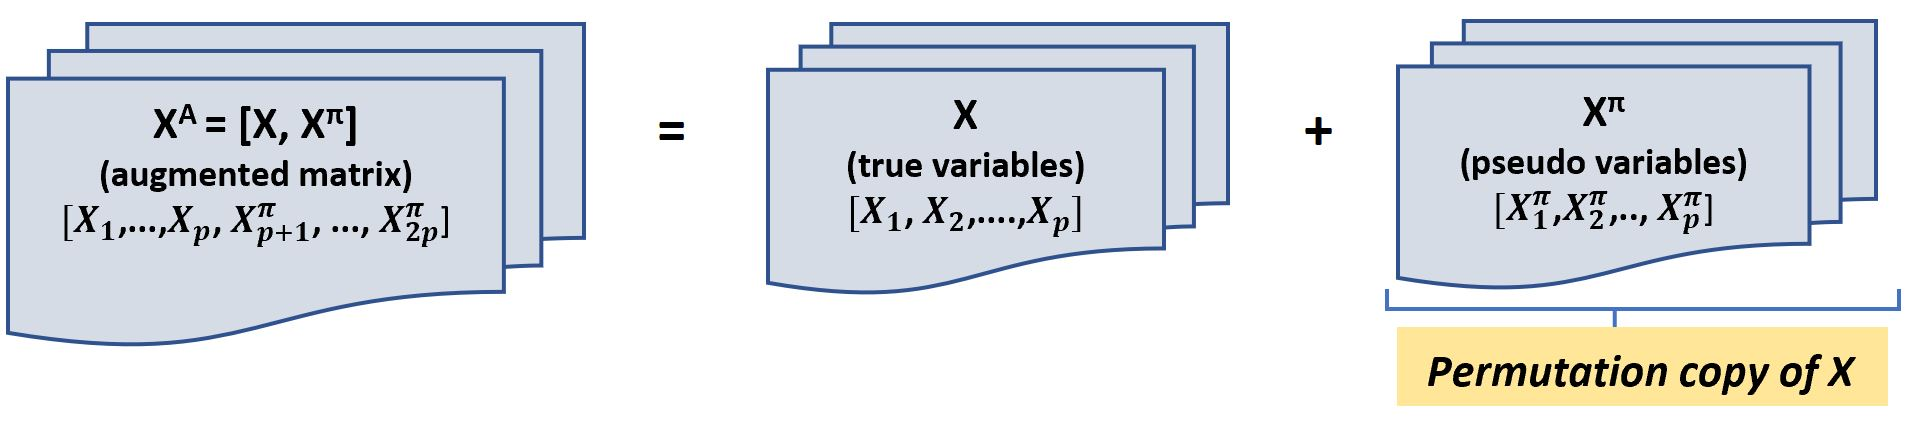
\includegraphics[scale=0.75]{PAT_model.jpg}
\caption{Permutation Assisted Tuning: The Augmented Model}%
{True set of predictor variables (dim: $\mathbf{x}_i\in\mathbb{R}^p$) is augmented with its permutation copy (dim: $\mathbf{x}_i^{\pi}\in\mathbb{R}^p$) to form an augmented design matrix $\mathbf{X}^A$ (dim: $\mathbf{x}_i^{A}\in\mathbb{R}^{2p}$).}
\label{fig:pat}
\end{figure}
\autoref{fig:pat} illustrates the idea of creating a permutation copy (set of pseudo-variables) from the original set of predictor variables and then augmenting them to increase the overall dimension of the predictor set while keeping the sample size constant. The new set of predictors for the augmented matrix can be written as $\mathbf{x}_i^A = ({x}_{i1}, ...,{x}_{ip}, {x^{\pi}}_{i(p+1)}, ...,{x^{\pi}}_{i(2p)})^T$ which are then grouped (based on the same common factors between the features used for the original predictor set) to now form a total of $2G$ groups of predictors. The predictor variables for the augmented matrix can be rewritten as $\mathbf{x}_i^A=(\mathbf{x}_{i1}, ..., \mathbf{x}_{iG},\mathbf{x^{\pi}}_{i1}, ..., \mathbf{x^{\pi}}_{iG})^T$ using the grouped variables $\mathbf{x}_{ig}\in\mathbb{R}^{\text{df}_g}$ where $g=1, ..., G$. Note that the grouping of the original predictor variables and that of the pseudo-variables remain the same, i.e. $[(1,2,..,G) = (G+1, G+2, ..., 2G)]$\par


The logistic group lasso estimator $\pmb{\hat\beta}_{\lambda}^A$ for this augmented design matrix is derived by minimizing the new objective function which is created by leveraging the equations \eqref{eq:2} and \eqref{eq:3}:
\begin{equation}\label{eq:4}
S_{\lambda}(\pmb{\beta}^A) = -\sum_{i=1}^{n}[y_i\eta_{\pmb{\beta}^A}(\mathbf{x}_i)-\log(1+\exp(\eta_{\pmb{\beta}^A}(\mathbf{x}_i))]+\lambda\sum_{g=1}^{2G} s(\text{df}_g)\|\beta_g^A\|_2^1
\end{equation}
In equation \eqref{eq:4}, the new tuning parameter $\lambda\ge 0$ controls the amount of penalization. Because of the way the pseudo-variables were constructed we know that the contribution of these variables should be absent from the model. Therefore, it is important that a preferred tuning parameter $\lambda$ should be able to rule out the coefficients that are assigned to the pseudo-variables making them active predictors (\cite{permassisttune}Yang \textit{et al.}, 2020). We consider the point $\lambda$ on the group lasso path at which the variable group $\mathbf{x}_{g}$ where $g\in 1,..,G$ remains in (or last enters in terms of decreasing $\lambda's$) the model but does not allow $\mathbf{x}_{g+1}$ where $g+1 \in G+1,...,2G$ to entire the model.\par
\begin{equation}\label{eq:pat_eq1}
W_g =\text{sup}\{\lambda: \hat{\beta}^A_g(\lambda)\ne 0\}; g=1,...,2G
\end{equation}
We set $W_g=0$ if a variable group does not enter the model even without the group lasso penalty (i.e., $\hat{\beta^A_g}(0)=0$ ). This new statistic $W_g$ can be viewed as an importance metric for the $g^{\text{th}}$ variable group, as an active variable tends to remain longer in the model as the penalty $\lambda$ increases compared to an inactive feature block.\par
Since these pseudo-variables are known to be inactive, a preferred tuning procedure should be able to rule out those $\lambda$ parameters that identify a pseudo-variable as active. Motivated by this, in terms of increasing $\lambda$'s, $C_{\pi}$ is defined as $C_{\pi}= \text{max}_{(G+1)\le g\le 2G}(W_g)$ as a benchmark to separate active variables from inactive ones. That leads to the following variable selection procedure
\begin{equation}\label{eq:pat_eq2}
\hat{S_{\pi}} = \{g: W_g>C_{\pi}, g=1,...,G\}
\end{equation}
In other words, only those original variables will be selected which have an importance metric $W_g$ greater than $C_{\pi}$, the maximum of importance metrics of all p pseudo-variables. In terms of decreasing $\lambda$'s, we iterate through all the $\lambda$ values until the point where pseudo-variables are assigned coefficients. That is $W_g\ne 0$ where $g\in G+1,...,2G$. We then use the $\lambda$ value prior to the $\lambda$ identified in the previous step. This technique guarantees that only the original active variables make into the model.\par
In equation \eqref{eq:pat_eq2}, $\hat S_{\pi}$ denotes the estimator of true active variables under a particular permutations $\pi$. Since the permutation copies will render different selection results, each time this variable selection model is executed, the $\hat S_{\pi}$ will be affected by the different permutations. The variable selection is stabilized by using different permutations iteratively and evaluating the frequency of the selected variables across the iterations. This technique of using Group Lasso with permutation assisted tuning henceforth would be referred to as the \lq Group Plasso' model.

\section{Selecting top network features}\label{sec:selectntw}
After prioritizing the network properties (feature blocks) we explore the top network features across the entire set of predictors and dive deeper to identify the significant aggregated feature from each of the feature blocks.
\subsection{Logistic Lasso Model set-up}\label{subsec:lasso}
The Lasso shrinkage and variable selection technique is used on the observed data to identify the top network features. The various features compete using the $L_1-$norm to produce a significant set of variables. Lasso is indifferent to any group structures created for the network properties. The objective function $S_{\lambda}(\pmb{\beta})$ defined using the negative log likelihood penalizes the absolute size of the $\pmb{\beta}$ coefficients based on the value of the tuning parameter $\lambda$. The logistic lasso estimator $\pmb{\hat\beta}_{\lambda}$ is derived by minimizing the objective function:
\begin{equation}\label{eq:5}
S_{\lambda}(\pmb{\beta}) = -l(\pmb{\beta})+\lambda\sum_{j=1}^{p} |\beta_j|
\end{equation}
where $l(.)$ is the log-likelihood function given as
\begin{equation}\label{eq:6}
l(\pmb{\beta})=\sum_{i=1}^{n}[y_i\eta_{\pmb{\beta}}(\mathbf{x}_i)-\log(1+\exp(\eta_{\pmb{\beta}}(\mathbf{x}_i))]
\end{equation}
and the penalty function is given as
\begin{equation}\label{eq:lasso penalty}
\lambda\sum_{j=1}^{p} |\beta_j|
\end{equation}
The tuning parameter $\lambda\ge 0$ controls the amount of penalization and is subject to $\sum_{j=1}^{p}|\beta_j|\le \theta(\lambda)$. The term $|\beta_j|$ in the penalty function implies the $L_1-$norm between the variables. For a given value of $\lambda$, a certain number of variables with non-zero coefficients can be selected. For a typical lasso solution path $\pmb{\hat\beta}_{\lambda}$, more variables can enter the model when $\lambda$ decreases. As the value of $\lambda$ increases, the irrelevant coefficients cease to exist leading to automatic variable selection.\par 
Optimal solution for the tuning parameter $\lambda$ can be deduced using different techniques. The most preferred approach is by using Cross-Validation. In our work we use Cross-Validation and the Permutation Assisted Tuning to derive the optimal $\lambda$. The latter approach has lower false positives (\cite{permassisttune}Yang \textit{et al.}, 2020) in comparison to the Cross-Validation approach.\par
Permutation assisted tuning for Lasso, also known as Plasso (\cite{permassisttune}Yang \textit{et al.}, 2020), works in the same manner as it does for Group Lasso. The only difference lies in the way that Group Lasso groups the original and the pseudo-variables, whereas, for Lasso the original and the pseudo-variables remain un-grouped. After augmentation of the permutation copy (pseudo-variables), the corresponding lasso problem is
\begin{equation}\label{eq:7}
\pmb{\beta}^A(\lambda) = \text{argmin}_{\pmb{\beta}^A}[-\sum_{i=1}^{n}[y_i\eta_{\pmb{\beta}^A}(\mathbf{x}_i)-\log(1+\exp(\eta_{\pmb{\beta}^A}(\mathbf{x}_i))]+\lambda\sum_{j=1}^{2p} |\beta_j^A|
\end{equation}
where $\pmb{\beta}^A = (\beta^A_1,..,\beta^A_p,\beta^A_{p+1},.., \beta^A_{2p})^T$ are the coefficients for both the $p$ original variables and $p$ pseudo-variables.\par
\subsection{Exclusive Lasso Model set-up}\label{subsec:exclusivelasso}
Exclusive Lasso (\cite{exclusv_lasso}Zhou,Jin and Hoi, 2010) is used to make inferences on the aggregated features from each feature block. It makes variables in the same group compete with every other variable within the same group and thus generates sparse solutions (within a feature block). The objective function $S_{\lambda}(\pmb\beta)$ for exclusive lasso is defined similarly to that of Group Lasso.
\begin{equation}\label{eq:8}
S_{\lambda}(\pmb\beta) = -l(\pmb\beta)+\lambda\sum_{g=1}^{G}s(\text{df}_g)\|\beta_g\|_1^2
\end{equation}
where the penalty term is given as 
\begin{equation}\label{eq:exclusvpenalty}
\lambda\sum_{g=1}^{G}s(\text{df}_g)\|\beta_g\|_1^2
\end{equation}
The term $\|\beta_g\|_1^2$ implies the $L_2-$norm among the groups and the $L_1-$norm within each group. The $l(.)$ is the log likelihood function for logistic regression and the function $s(.)$ is used to rescale the penalty with respect to the dimensionality of the parameter vector $\beta_g$ (\cite{grouporigin}Yuan and Lin, 2006). The logistic exclusive lasso estimator $\pmb{\hat\beta}_{\lambda}$ is derived by minimizing the objective function from the equation \eqref{eq:8}. The tuning parameter $\lambda\ge 0$ controls the amount of penalization of the model and is subject to $\sum_{g=1}^{G}\|\beta_g\|^{2}_{1}\le \theta(\lambda)$, where $\theta(.)$ is some function of $\lambda$.\par
The optimal value of the tuning parameter $\lambda$ can be derived by using Cross-Validation. However, unlike Lasso and Group Lasso, permutation assisted tuning cannot be used to deduce lambda for Exclusive Lasso. Since exclusive lasso applies the $L_2-$norm across all groups (generates dense solution across groups and sparse solution within a group), it is bound to assign coefficients to all groups. As a result, when pseudo-variables are added to the model, exclusive lasso in all situations will generate coefficients for the groups containing the pseudo-variables. Hence, we can never achieve the desired model by excluding the groups containing the pseudo-variable in this case. Therefore, we will limit our usage to Cross-Validation approach for finding $\lambda$ in the Exclusive Lasso model.\par






